\subsection{Using the Graticule Creator Plugin}

The graticule creator allows to create a ``grid'' of points, line or
polygons to cover our area of interest. All units must be entered in
decimal degrees. The output is a shapefile which can be projected on the
fly to match your other data.

\begin{figure}[ht]
\begin{center}
  \caption{Create a graticule layer}\label{fig:graticule}\smallskip
  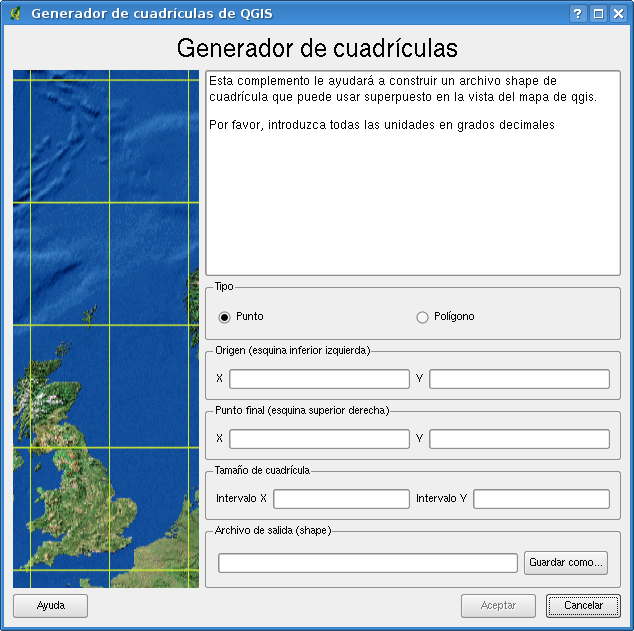
\includegraphics[scale=0.5]{graticule}
\end{center}
\end{figure}

Here is an example how to create a graticule:

\begin{enumerate}
\item Make sure the plugin is loaded.
\item Click on the \textsl{Graticule Creator} tool on the plugins toolbar.
\item Choose the type of graticule you wish to create: point, line or
  polygon.
\item Enter the latitude and longitude for the lower left and upper right
  corners of the graticule.
\item Enter the interval to be used in constructing the grid. You can
  enter different values for the X and Y directions (longitude, latitude)
\item Choose the name and location of the shapefile to be created.
\item Click \textsl{OK} to create the graticule and add it to the map
  canvas.
\end{enumerate} 


